\documentclass[a4paper,10pt]{article} % Default font size and paper size

\usepackage[T1]{fontenc}
\usepackage{multicol}
\usepackage{marvosym}
\usepackage{wasysym}
\usepackage{multirow}
\usepackage{blindtext}
\usepackage{polyglossia} 
\usepackage{xunicode,xltxtra,url,parskip}
\usepackage[usenames,dvipsnames]{xcolor}
\usepackage{enumitem}
\setitemize{noitemsep,topsep=0pt,parsep=1pt,partopsep=0pt}
\setlength{\textfloatsep}{-3cm}
\usepackage{marvosym}

\definecolor{grays}{rgb}{0.33, 0.33, 0.33}
\definecolor{grees}{rgb}{0.60, 0.67, 0.12}
\definecolor{blue}{rgb}{0.085, 0.234, 0.4}
\setdefaultlanguage[spelling=modern]{russian}
\setotherlanguage{english}
\usepackage{fontspec}

\setmonofont{[cmuntt.otf]}
\newfontfamily\cyrillicfont[  
	BoldFont        = [cmunbx.otf],
    ItalicFont      = [cmunti.otf],
    BoldItalicFont  = [cmunbx.otf],
    SmallCapsFont   = [cmunrm.otf],
    Mapping         = tex-text
]{[cmunrm.otf]}

% Параметры страницы
\textheight=27cm
\textwidth=19.5cm
\oddsidemargin=-2mm
\evensidemargin=-5mm
\marginparwidth=36pt
\topmargin = -3cm
\footnotesep=3ex
\hoffset = -1.5cm
\tolerance 3000
% подавить эффект "висячих стpок"
\clubpenalty=10000
\widowpenalty=10000

\usepackage{hyperref} % Required for adding links	and customizing them
\definecolor{linkcolour}{rgb}{0,0.0,0.0} % Link color
\hypersetup{colorlinks,breaklinks,urlcolor=linkcolour,linkcolor=linkcolour} % Set link colors throughout the document

\usepackage{titlesec} % Used to customize the \section command
\titleformat{\section}{\Large\scshape\raggedright}{}{0em}{}[\titlerule] % Text formatting of sections
\titlespacing{\section}{0pt}{3pt}{3pt} % Spacing around sections
\title{ashuha_resume}

\begin{document}

\pagestyle{empty} % Removes page numbering

\font\fb=''[cmr10]'' % Change the font of the \LaTeX command under the skills section
\oddsidemargin=0pt 		% отступ от левого края
%----------------------------------------------------------------------------------------
%	NAME AND CONTACT INFORMATION
%----------------------------------------------------------------------------------------

\begin{center}
	{\huge Arsenii Ashukha}
\end{center}
\begin{center}
\textcolor{gray}{
Moscow, Russia $\bullet$ 
\Letter~\textcolor{gray}{\texttt{ars.ashuha@gmail.com}} $\bullet$ \href{https://ars-ashuha.ru/}{\textcolor{gray}{\texttt{ars-ashuha.ru}}} $\bullet$
23 years old \smiley} 

\end{center}
\setlength{\columnsep}{-330pt}
\begin{multicols}{2}
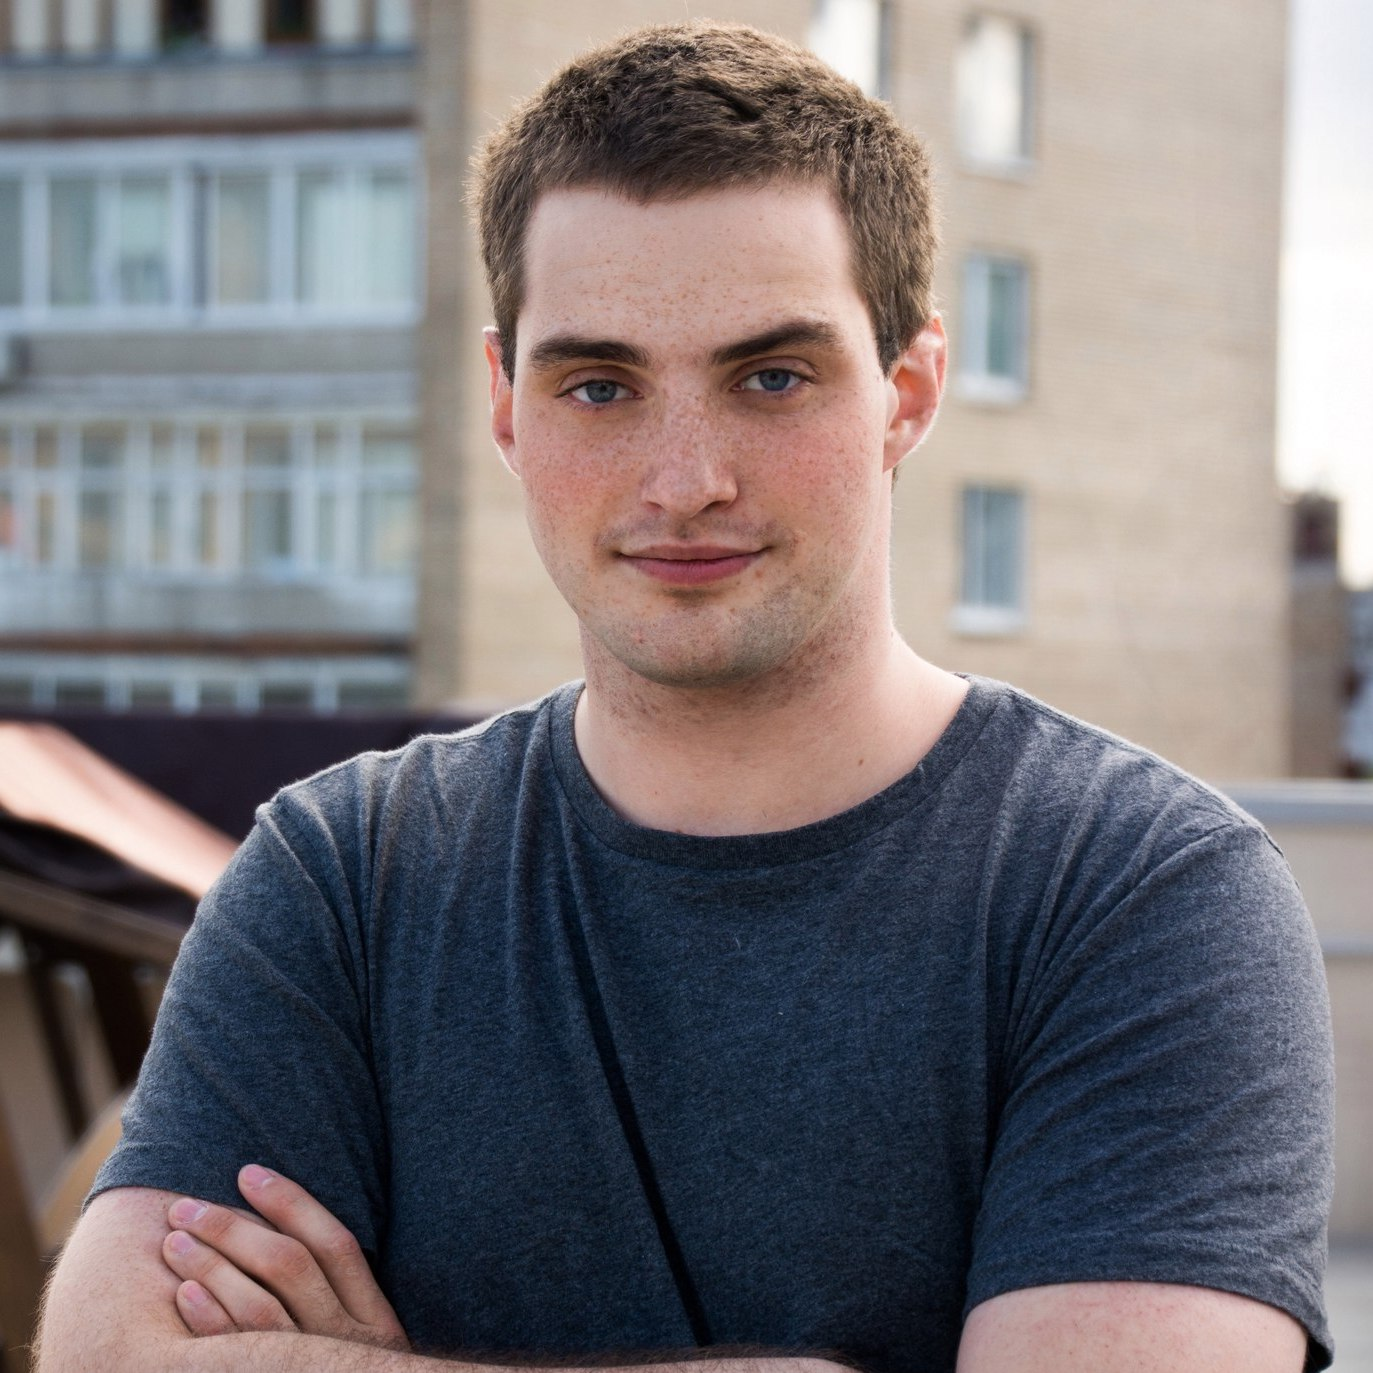
\includegraphics[scale=0.07]{../images/avatar_v3}

\section{Summary}
 \vspace{-0.2cm}

I am a second year Master Student at MIPT also I do research at \href{bayesgroup.ru}{Bayes Group} under supervision of prof. Dmitry Vetrov. My research is focused on Bayesian regularization of deep neural nets. At MIPT, MSU, HSE I teach several Machine Learning courses. To see the publication list visit my scholar profile.

\vspace{0.2cm}
\textbf{Skills}: Machine Learning, Deep Learning, Bayesian ML, Python, Hadoop, Linux, Fluent English

\end{multicols}

%----------------------------------------------------------------------------------------
%	EDUCATION
%----------------------------------------------------------------------------------------

\section{Education}

\begin{tabular}{rp{14cm}c}	
	\textbf{2015 -  2017} & Master, \emph{Machine Learning}, \href{https://mipt.ru/english}{Moscow Institute of Physics and Technology}, GPA: 9.0/10.0& \multirow{2}{*}{
\includegraphics[scale=0.15]{img/mipt}}\\
	\textsc{Thesis} & \emph{Variational Dropout Sparsifies DNNs}, Supervisor: \href{https://scholar.google.ru/citations?user=7HU0UoUAAAAJ&hl=en}{Prof. D. Vetrov (\texttt{\textbf{HSE}})}, \href{https://ru.linkedin.com/in/alexey-dral}{A. Dral (\texttt{\textbf{MIPT}})}
\end{tabular}

\begin{tabular}{rp{14cm}c}	
	\textbf{2015 -  2016} & Irregular Student, \emph{Machine Learning}, \href{https://yandexdataschool.com/}{Yandex School of Data Analysis}, GPA: 4.8/5.0& \multirow{2}{*}{~~
\includegraphics[scale=0.25]{img/shad}}\\
	\textsc{Result}~& \emph{Six courses were passed and the favorites are Bayesian ML, Deep Learning, Machine Learning}
\end{tabular}

\begin{tabular}{rp{14cm}c}	
\textbf{2011 -  2015} & Bachelor, \emph{Computer Science}, \href{http://www.bmstu.ru/en/}{Bauman Moscow State Technical University}, GPA: 3.7/5.0 & \multirow{2}{*}{~~~~~
\includegraphics[scale=0.012]{img/bmstu}}\\
\textsc{Thesis} &\emph{\href{https://github.com/ars-ashuha/bigram-anchor-words}{\textcolor{black}{Building of Uncorrelated Kernels for Topic Models}}}, Supervisor:  \href{https://scholar.google.ru/citations?user=FKkWXLkAAAAJ&hl=en}{\textcolor{black}{N. Loukachevitch~(\texttt{\textbf{MSU}})}}
\end{tabular}



\section{Experience}


\begin{tabular}{r|p{11.5cm}c}
\textbf{Mar 2017 - Now~~~~~~} & 
\textbf{HSE}, Moscow --- Intern Researcher  at Lab of DL and Bayesian ML &
\multirow{2}{*}{	\vspace*{+5cm}
\includegraphics[scale=0.032]{img/hse}} \\
~~~~~~~~~~~&  
\footnotesize{  \vspace{-0.25cm}
	\begin{itemize}
		\item[-] Research on efficient training of DNNs all details are hidden under NDA
	\end{itemize}
\scriptsize{
	\emph{Chief}: 
	Dmitriy Vetrov
	(\href{mailto:vetrovd@yandex.ru}{\textcolor{gray}{vetrovd@yandex.ru}})}
	\vspace{-0.1cm}} & 
\\
\multicolumn{2}{c}{}\\


\textbf{Jun 2016 - Aug 2016} & 
\textbf{Yandex}, Moscow --- Intern at Music Deep Learning Group &
\multirow{2}{*}{
\includegraphics[scale=0.015]{img/yandex}} \\ 
\textcolor{gray}{3 month}~~~~~~~~~~~&  \footnotesize{
  
  \vspace{-0.25cm}
  \begin{itemize}
      \item[-] Searching similar tracks and building recommendation features using DNN
  \end{itemize}
\scriptsize{
	\emph{Chief}:  
	Eugene Krofto
	(\href{mailto:singleton@yandex-team.ru}{\textcolor{gray}{singleton@yandex-team.ru}})}
  \vspace{-0.1cm}
} & 
\\
\multicolumn{2}{c}{}\\

\textbf{Dec 2013 - Feb 2016} &  
\textbf{Rambler}, Moscow --- R\&D Engineer at Machine Learning Group  &
\multirow{1}{*}{
\includegraphics[scale=0.1]{img/ramblerco}}\\ 
\textcolor{gray}{2 year 1 month p/t}~~ &  \footnotesize{
  \vspace{-0.25cm}
  \begin{itemize}
      \item[-] Improving the quality and performance of user classification using browser history
  	  \item[-] Recommendations system for the news posts on \texttt{rambler.ru}
  \end{itemize}
	\scriptsize{
	\emph{Chief}:  
	\href{https://ru.linkedin.com/in/pavel-klemenkov-7a88a956}{Pavel Klemenkov} 
	(\href{mailto:pklemenkov@gmail.com}{\textcolor{gray}{pklemenkov@gmail.com}}),
	\href{https://ru.linkedin.com/in/anton-gorokhov-2959482}{Anton Gorokhov}
	(\href{mailto:anton.gorokhov@gmail.com}{\textcolor{gray}{anton.gorokhov@gmail.com}})}
  \vspace{-0.1cm}
} & 
\\
\multicolumn{2}{c}{}\\

\textbf{Jun 2013 - Aug 2013} & 
\textbf{Rambler}, Moscow --- Intern at Search Group&
\multirow{1}{*}{
\includegraphics[scale=0.1]{img/ramblerco}}\\ 
\textcolor{gray}{3 month}~~~~~~~~~~~& 
\footnotesize{

\vspace{-0.25cm}
\begin{itemize}
	\item[-] Users query classification to show a mixing in search results
\end{itemize}
\scriptsize{
	\emph{Chief}:  
Max Karpenko
(\href{mailto:v3dmax@gmail.com}{\textcolor{gray}{v3dmax@gmail.com}})}
\vspace{-0.1cm}
}& 
\\
\end{tabular}

\section{Teaching}
\begin{itemize}
	\item \textbf{Feb 2016 - Feb 2017:} Practical Lecturer of  \href{https://ml-mipt.github.io/}{\texttt{Machine Learning course}} at  MIPT (parts 1,2)
	\item \textbf{Sep 2016 - Now:} Lecturer of several classes of Deep Learning courses at \href{https://goo.gl/3wXB4f}{MSU} and \href{https://github.com/yandexdataschool/HSE_deeplearning}{HSE}
	\item  \textbf{Oct 2016 - Now:}  Lecturer of DL part of \href{https://vk.com/data_mining_in_action}{Data Mining in Action course}, \href{https://www.youtube.com/channel/UCop3CelRVvrchG5lsPyxvHg}{YouTube records  in Russian \frownie}
	\item  \textbf{Feb 2017 - Now:}  Lecturer of DL part in \href{https://ml-mipt.github.io/}{Machine Learning course} at MIPT
	\item  \textbf{Feb 2017 - Now:}  Co-head of Scientific Machine Learning seminar for MIPT and HSE \href{https://yandexdataschool.com/}{Yandex} students
\end{itemize}

\end{document}

